%!TEX program = xelatex 
% !BIB program = biber
%%%%%%%%%%%%%%%%%%%%%%%%%%%%%%%%%%%%%%%%%%%%%%%%%%
% 载入模版
%
% 载入 hutbthesis.cls文件定义的模板
%%%%%%%%%%%%%%%%%%%%%%%%%%%%%%%%%%%%%%%%%%%%%%%%%%

\documentclass[AutoFakeBold]{hutbthesis}

\addbibresource{content/reference.bib}

%%%%%%%%%%%%%%%%%%%%%%%%%%%%%%%%%%%%%%%%%%%%%%%%%%
% 基本信息
%
% 用户自行输入标题、作者等基本信息
% 都存储在\content\info.tex文件中
%%%%%%%%%%%%%%%%%%%%%%%%%%%%%%%%%%%%%%%%%%%%%%%%%%
%!TEX root = ../hutbthesis_main.tex
% 文章信息
\titlecn{湖南工商大学学位论文 } 
\titleen{Hunan University of Technology and Business Thesis \LaTeX{} Template v0.1}


%\minormajor{通信工程}
%\interestmajor{通信工程}
\author{张瀚驰}
\subsupervisor{}
\studentid{2123030023}
\priormajor{大数据与人工智能}
\myclass{数智2101班}
\supervisor{王海东\ 教授}
\department{人工智能与先进计算学院}
\thesisdate{year=2024, month=12}

%以下的对本科生没有用
\clcnumber{TP391} 				% 中图分类号 Chinese Library Classification
\schoolcode{10533}			% 学校代码
\udc{004.9}						% UDC
\academiccategory{学术学位}	% 学术类别



\begin{document}
%%%%%%%%%%%%%%%%%%%%%%%%%%%%%%%%%%%%%%%%%%%%%%%%%%
% 封面绘制
%
% 1.5版本重新编写了封面绘制宏,并用latex使用者更习惯的
% \maketitle代替之前的\makecoverpage
%%%%%%%%%%%%%%%%%%%%%%%%%%%%%%%%%%%%%%%%%%%%%%%%%%
\maketitle

%\declarationzh

% 启用大罗马字母进行编号
\frontmatter
% 设置页眉和页脚

%%!TEX root = ../csuthesis_main.tex
% 文章信息
\titlecn{湖南工商大学大学学位论文 \LaTeX{} }
\titleen{Central South University Thesis \LaTeX{} }

\priormajor{}
\minormajor{}
\interestmajor{}
\author{张瀚驰}
\supervisor{王海东\ 教授}
\subsupervisor{}
\department{人工智能与先进计算学院}
\studentid{2123030023}
\thesisdate{year=2024,month=12}
\myclass{大数据与人工智能}


%以下的对本科生没有用
\clcnumber{TP391} 				% 中图分类号 Chinese Library Classification
\schoolcode{10533}			% 学校代码
\udc{004.9}						% UDC
\academiccategory{学术学位}	% 学术类别

%!TEX root = ../hutbthesis_main.tex

\begin{declarationzh}
		
本人郑重声明:所呈交的本科毕业设计 \uline{ 湖南工商大学学位论文 \LaTeX{} 模板使用示例 v0.1 } 是本人在指导老师的指导下,独立进行研究工作所取得的成果,成果不存在知识产权争议,除文中已经注明引用的内容外,本设计不含任何其他个人或集体已经发表或撰写过的作品成果。
对本设计做出重要贡献的个人和集体均已在文中以明确方式标明。本人完全意识到本声明的法律结果由本人承担。
	
	\vspace{30pt}
	\begin{tabular}{ll}
		%\renewcommand{\arraystretch}{2}
		\hspace{240pt} \makebox[4em][s]{作者签名:} & \underline{\makebox[100pt][c]{  }} \\
		\hspace{240pt} \makebox[4em][s]{日\qquad 期:}	 &
		\underline{\makebox[100pt][c]{\qquad 年\quad 月\quad   日 }} \\
	\end{tabular}

	
	
\end{declarationzh}

%%%%%%%%%%%%%%%%%%%%%%%%%%%%%%%%%%%%%%%%%%%%%%%%%%
% 中文摘要
%
% 存储在\content\abstractzh.tex文件中
%%%%%%%%%%%%%%%%%%%%%%%%%%%%%%%%%%%%%%%%%%%%%%%%%%
%!TEX root = ../csuthesis_main.tex
% 设置中文摘要
\keywordscn{行人导航\quad 强化学习\quad 虚拟仿真\quad Carla平台\quad 路径规划\quad 避障}
%\categorycn{TP391}
\begin{abstractzh}

交通管理中行人导航关键技术的研究在智慧城市交通系统智能化的背景下,有着重要的意义。基于规则模型或是简单路径规划的方法显然无法适应交通管理的新需求,强化学习作为自适应学习最优策略的方法,具有在动态环境下决策的优势。本文设计基于虚拟引擎和carla平台的行人导航系统,利用强化学习进行路径规划和避障规划,以实现提高避障能力和路径规划效率的目的,在一定程度上能够拓展强化学习在智能交通系统中的应用范畴,并为智慧城市的发展提供技术参考。在快速城市化发展的当下,交通系统智能化的方向关键在于效率与安全,行人导航相关技术研究与应用虽然满足了交通管理的基本需求,但面对更加复杂的动态环境,研发适应性更强的行人导航系统极为必要。在不确定和动态环境下进行决策,强化学习具有较好的应对能力。本文在虚拟仿真技术的基础上进行行人导航系统创新设计,基于虚幻引擎和carla平台搭建了虚拟导航环境,可实时优化路径规划方案和避障策略。之后在多个系统仿真场景进行了有效性实验,诸如导航精度、避障能力、路径规划效率评估等等,验证了系统所基于强化学习的导航系统对于系统动态环境仍具有较为优秀的性能,提高了导航感受和交通效率。研究成果在强化学习在智能交通领域的应用研究上为智慧城市建设提供技术支撑,随着技术的进步和交通需求量的增加,基于强化学习的行人导航系统在城市交通领域将会得到普遍应用。

\end{abstractzh}


%%%%%%%%%%%%%%%%%%%%%%%%%%%%%%%%%%%%%%%%%%%%%%%%%%
% 英文摘要
%
% 存储在\content\abstracten.tex文件中
%%%%%%%%%%%%%%%%%%%%%%%%%%%%%%%%%%%%%%%%%%%%%%%%%%
%!TEX root = ../csuthesis_main.tex
\keywordsen{Pedestrian navigation, Reinforcement learning, Virtual simulation, Carla platform, Path planning, Obstacle avoidance}
\begin{abstracten}

As urban traffic systems progress towards enhanced intelligence, the research and development of pedestrian navigation and control systems have gained increasing importance in traffic management and smart city infrastructure development. Traditional pedestrian guidance methods, often relying on rule-based models or basic path planning algorithms, are frequently insufficient in adapting to the dynamic and complex nature of urban environments.This limitation presents a hurdle in meeting the real-time and intelligent requirements of modern traffic systems. Recently, reinforcement learning, an AI technique proficient in adaptive learning of optimal strategies, has emerged as a potent tool for addressing decision-making challenges in dynamic environments.This specific research effort presents a new pedestrian navigation system based on Unreal Engine and Carla platform. It combines virtual simulation with reinforcement learning principles to enhance path planning and obstacle avoidance through adaptive learning.To comprehensively evaluate and compare its performance with traditional path planning algorithms, the system conducted a series of experiments in various simulation environments. The experimental results show that the pedestrian navigation system based on reinforcement learning significantly improves the efficiency of pedestrian obstacle avoidance and path planning in dynamic urban landscapes. This research not only expands the application scope of reinforcement learning in intelligent traffic systems but also provides innovative technical solutions crucial for the future development of smart cities.

\end{abstracten}



%%%%%%%%%%%%%%%%%%%%%%%%%%%%%%%%%%%%%%%%%%%%%%%%%%
% 目录
%
% 使用重定义的tableofcontents宏绘制目录
% 满足学校的样式要求
%%%%%%%%%%%%%%%%%%%%%%%%%%%%%%%%%%%%%%%%%%%%%%%%%%
\tableofcontents


% 启用数字编号,改为第 x 页  共 x 页格式
\mainmatter

%%%%%%%%%%%%%%%%%%%%%%%%%%%%%%%%%%%%%%%%%%%%%%%%%%
% 正文
%
% 存储在\content\content.tex文件中
%%%%%%%%%%%%%%%%%%%%%%%%%%%%%%%%%%%%%%%%%%%%%%%%%%
% 正文
%%!TEX root = ../hutbthesis_main.tex

%子章节为了便于查找和修改,建议通过input拆分文件

%%%%%%%%%%%%%%%%%%%%%%%%%%%%%%%%绪论%%%%%%%%%%%%%%%%
\chapter{选题背景与价值}

\section{选题价值}

智慧城市与智能交通发展背景下行人导航与控制系统在现代交通管理中作用重要。行人作为城市交通系统的重要组成部分其行为具有显著随机性和多样性给传统交通管理和路径规划方法带来诸多挑战,行人导航系统研究旨在通过实时路径优化与智能调控提升行人交通安全与出行效率。但传统导航方法多基于规则模型主要依赖静态预设参数,难以应对复杂动态环境中行人行为的快速变化,比如面对突发障碍物或密集交通流动时传统算法常无法快速调整路径规划或实时优化决策进而影响导航系统可靠性与安全性。

近年来人工智能技术快速发展,强化学习作为数据驱动的决策优化方法为行人导航领域提供全新思路,其通过智能体与环境交互学习最优策略能在动态环境中实现实时决策优化,特别适用于非线性非结构化的复杂场景。不过仅依靠强化学习技术难以全面解决行人导航问题,现实环境中数据采集的高成本高风险特性在实际应用中极大限制了强化学习的训练与推广。

本研究基于 Carla 利用虚幻引擎这一高仿真度虚拟场景构建平台提供了解决实际环境数据采集困难的理想工具,该引擎既能生成复杂多样的动态环境也能模拟真实场景中行人行为的随机性和多样性,为强化学习智能体的训练与测试提供安全低成本的实验平台。如通过虚幻引擎模拟十字路口复杂交通场景可逼真再现行人与车辆的动态交互,为强化学习算法的优化与验证创造实验条件,且其支持生成视觉、惯性、语义信息等多种传感器数据进一步丰富了强化学习的训练数据来源。

本研究结合虚拟仿真技术和强化学习算法解决行人导航核心问题,包括精准建模动态环境下行人行为,行人行为受交通信号、周围车辆动态变化及其他行人行为等多种因素影响,建立能真实反映不同环境中行人决策逻辑的高精度行人行为模型是首要难题;高效结合虚拟仿真与强化学习,强化学习有效性依赖训练环境质量,虚幻引擎仿真能力为训练高效智能体提供可能,但设计能充分利用虚幻引擎生成的多样化数据的高效强化学习算法亟待解决;平衡路径规划效率与行人安全性,行人导航系统要提高路径规划效率并优先考虑行人安全,如在交通高峰期复杂场景中找到安全高效路径是研究重点。

智慧交通系统发展对行人导航系统提出更高要求,既需与车辆、交通信号灯等其他交通参与者无缝协作以优化交通系统运行效率,随着多智能体技术发展,行人导航系统研究也从单一智能体优化转向多智能体协作,通过多智能体协同作用提升导航效率与安全性是未来重要研究方向。

本研究引入虚幻引擎仿真能力与强化学习自适应策略优化能力试图突破上述问题,虚幻引擎的逼真场景和多样化数据为复杂行为建模和智能体训练提供支持,强化学习算法自适应优化能力使智能体可快速适应复杂动态环境变化,两者结合能为行人导航系统提供新理论和技术支撑,在智能交通、自动驾驶和城市规划等领域有广泛应用潜力。

\section{文献综述}

近年来强化学习与虚拟仿真技术在智能交通和行人导航领域研究取得显著进展,从强化学习在行人导航中的应用、虚幻引擎在智能体训练中的作用以及行人导航的挑战与发展趋势三方面进行综述。

\subsection{强化学习在行人导航中的应用}

强化学习(Reinforcement Learning, RL)是一种通过智能体与环境交互学习最优策略的方法,近年来在交通系统优化和行人导航中得到了广泛应用。与传统路径规划方法相比,强化学习不仅可以应对动态环境,还能通过不断训练提高系统性能,展现了较高的自适应性和优化能力。强化学习技术在交通信号控制取得重要成果,钱立军等\cite{qian2024sac}基于 SAC 算法优化多交叉口交通信号控制提升交通通行效率,为动态环境复杂信号调度提供新思路,Wei 等\cite{wei2021survey}综述强化学习在交通信号控制研究进展指出深度强化学习(Deep Reinforcement Learning, DRL)解决非线性优化问题优势适用于实时动态交通场景;在路径规划领域应用广泛,陶幸等\cite{tao2024motion}提出基于惯性传感器免对准动作捕捉方法为动态场景行人行为建模提供技术支持,Chen 等\cite{chen2018ionet}结合深度学习与强化学习技术设计基于因果推理路径优化方法引入因果关系提升智能体在动态环境适应能力;深度强化学习为路径规划研究注入新动力,Mnih 等\cite{mnih2013dqn}首次提出深度 Q 学习(Deep Q - Learning, DQN)算法将深度神经网络引入强化学习框架提升其在高维状态空间表现能力;在多智能体协作问题广泛研究,Lian 等\cite{lian2023inverseql}设计基于离线 Q 学习多智能体协作算法解决复杂动态场景全局优化问题。

\subsection{虚幻引擎在智能体训练中的作用}

虚幻引擎(Unreal Engine)作为高仿真虚拟场景构建工具为复杂动态环境下强化学习算法训练和验证提供高效实验平台,借由强大虚拟仿真能力和多样化场景支持成为智能体训练测试重要工具。

1. \textbf{虚幻引擎在视觉导航研究中的应用:} 虚幻引擎在视觉导航研究应用广泛,Mourikis 等\cite{mourikis2007msckf}结合虚幻引擎构建视觉惯性导航系统并通过多状态约束卡尔曼滤波(MSCKF)算法优化路径规划,Campos 等\cite{campos2021orbslam3}提出的 ORB-SLAM3 算法利用虚拟场景数据显著提升视觉建图与定位的鲁棒性和精度为复杂动态环境中的导航提供有力支持。

2. \textbf{虚幻引擎在路径规划中的贡献:} 虚幻引擎于路径规划研究表现重要作用,Guo 等\cite{guo2020pdr}结合虚幻引擎动态仿真能力提出基于 PDR/UWB 融合的导航系统用于复杂环境行人路径优化,Wang 等\cite{wang2023llio}通过虚幻引擎构建高仿真交通场景训练强化学习智能体路径规划策略验证其在强化学习训练中的高效性和低成本特性。

3. \textbf{虚幻引擎与目标检测的结合:} 虚幻引擎还被用于目标检测与路径规划结合研究,Redmon 等\cite{redmon2017yolo9000}通过虚幻引擎生成增强数据训练 YOLO 目标检测模型提高目标检测在复杂场景中的表现能力,Simonyan 和 Zisserman 等\cite{simonyan2014action}进一步研究虚幻引擎对深度学习模型的优化作用为复杂交通场景下的行为预测提供理论支持。 

4. \textbf{虚幻引擎在多智能体协作中的应用:} 虚幻引擎的仿真能力在多智能体协作研究中广泛应用,Bochkovskiy 等\cite{bochkovskiy2020yolov4}开发基于虚幻引擎的交通流量仿真工具验证多智能体协作算法有效性,Campos 等\cite{campos2021orbslam3}通过虚拟场景数据验证智能体在多智能体协作场景中的优化表现为行人导航系统的多智能体研究提供重要支持。

虚幻引擎为强化学习算法设计训练与验证提供有力支持,在视觉导航路径规划与多智能体协作中的应用展现巨大潜力。

\subsection{行人导航的挑战与发展趋势}

行人导航技术虽取得显著进展但在复杂动态环境中仍存复杂行为建模、动态环境适应性及多智能体协作优化等诸多挑战。

1. \textbf{行人行为的复杂建模:} 行人行为具显著多样性与随机性,赵靖等\cite{zhao2014crossing}提出基于动态信号优化的行人过街模型通过行为建模提升信号控制效率与安全性,Foxlin 等\cite{foxlin2005tracking}设计基于惯性传感器的行人轨迹跟踪方法为复杂行为建模提供技术支持。

2. \textbf{动态环境的实时适应:} 动态环境不确定性对导航系统提出更高要求,Herath 等\cite{herath2020ronin}通过视觉信号优化路径规划使智能体实时适应动态障碍物变化,Wang 等\cite{wang2013densetrajectory}提出基于强化学习的信号优化方法在动态环境中提升系统鲁棒性。

3. \textbf{多智能体协作的优化:} 复杂交通场景中多智能体协作优化问题尤为重要,Lian 等\cite{lian2023inverseql}通过强化学习实现多智能体高效协作提高全局路径规划效率,Campos 等\cite{campos2021orbslam3}利用虚幻引擎验证多智能体协作优化算法在复杂场景中的应用价值。

4. \textbf{未来研究趋势:} 未来行人导航研究将朝以下方向发展:基于多源数据的复杂行为建模与优化;提升强化学习智能体在动态环境中的泛化能力;多智能体协作优化在虚拟仿真环境中的深度应用。

%%%%%%%%%%%%%%%%%%%%%%%%%%%%%%%%绪论%%%%%%%%%%%%%%%%

%%%%%%%%%%%%%%%%%%%%%%%%%%%%%%%%图像插入示例%%%%%%%%%%%%%%%%
%!TEX root = ../../csuthesis_main.tex
\chapter{图表示例}

\section{图片与布局}

\subsection{插图}

图片可以通过\cs{includegraphics}指令插入,我们建议模板使用者将文章所需插入的图片源问卷放置在 images 目录中,
另外,矢量图片应使用PDF格式,位图照片则应使用JPG格式(LaTeX不支持TIFF格式)。具有透明背景的栅格图可以使用PNG格式。

下面是一个简单的插图示例。

\begin{figure}[hbt]
    \centering
    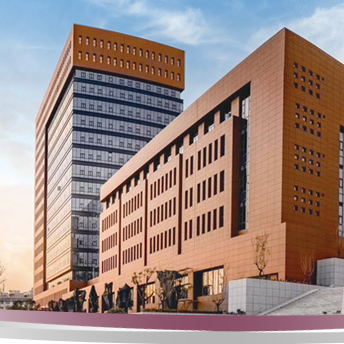
\includegraphics[width=0.3\linewidth]{hutb_building.png}
    \caption{插图示例}
    \label{f.example}
\end{figure}


如果一个图由多个分图(子图)组成,应通过(a),(b),(c)进行标识并附注在分图(子图下方)。
目前子图标识不居中问题没有解决,预计下个版本修复。

\subsection{横向布局}

模板提供常见的图片布局,比如单图布局\ref{f.example},另外还有横排布局如下:

\begin{figure}[!htb]
    \centering
    \begin{subfigure}[t]{0.24\linewidth}
        \begin{minipage}[b]{1\linewidth}
        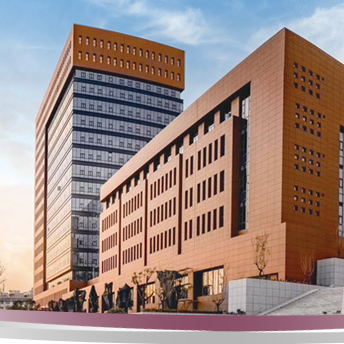
\includegraphics[width=1\linewidth]{hutb_building.png}
        \caption{test}
        \end{minipage}
    \end{subfigure}
    \begin{subfigure}[t]{0.24\linewidth}
        \begin{minipage}[b]{1\linewidth}
        \includegraphics[width=1\linewidth]{hutb_eim.png}
        \caption{test}
        \end{minipage}
    \end{subfigure}
    \begin{subfigure}[t]{0.24\linewidth}
        \begin{minipage}[b]{1\linewidth}
        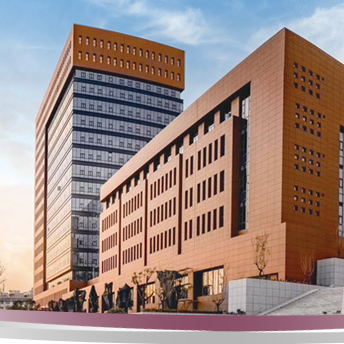
\includegraphics[width=1\linewidth]{hutb_building.png}
        \caption{test}
        \end{minipage}
    \end{subfigure}
    \begin{subfigure}[t]{0.24\linewidth}
        \begin{minipage}[b]{1\linewidth}
        \includegraphics[width=1\linewidth]{hutb_eim.png}
        \caption{test}
        \end{minipage}
    \end{subfigure}
    \caption{图片横排布局示例}
    \label{f.row}
\end{figure}

\section{纵向布局}

纵向布局如图\ref{f.col}

\begin{figure}[!htb]
    \centering
    \begin{subfigure}[t]{0.15\linewidth}
        \captionsetup{justification=centering} %ugly hacks
        \begin{minipage}[b]{1\linewidth}
        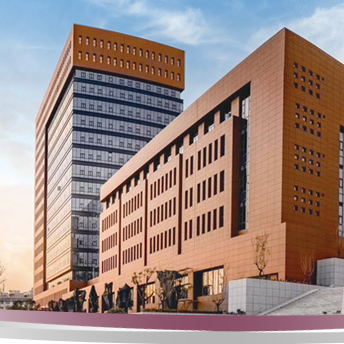
\includegraphics[width=1\linewidth]{hutb_building.png}
        \caption{test}
        \end{minipage}
    \end{subfigure}\\
    \begin{subfigure}[t]{0.15\linewidth}
        \captionsetup{justification=centering} %ugly hacks
        \begin{minipage}[b]{1\linewidth}
        \includegraphics[width=1\linewidth]{hutb_eim.png}
        \caption{test}
        \end{minipage}
    \end{subfigure}
    \caption{图片纵向布局示例}
    \label{f.col}
\end{figure}

\section{竖排多图横排布局}

\begin{figure}[!htb]
    \centering
    \begin{subfigure}[t]{0.13\linewidth}
        \captionsetup{justification=centering} 
        \begin{minipage}[b]{1\linewidth}
        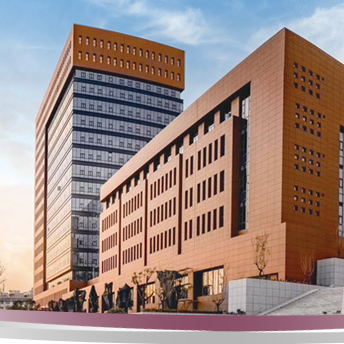
\includegraphics[width=1\linewidth]{hutb_building.png} 
        \vspace{-1ex} \vfill
        \includegraphics[width=1\linewidth]{hutb_eim.png}
        \caption{aaa}
        \end{minipage}
    \end{subfigure}
    \begin{subfigure}[t]{0.13\linewidth}
        \captionsetup{justification=centering} 
        \begin{minipage}[b]{1\linewidth}
        \includegraphics[width=1\linewidth]{hutb_eim.png} 
        \vspace{-1ex} \vfill
        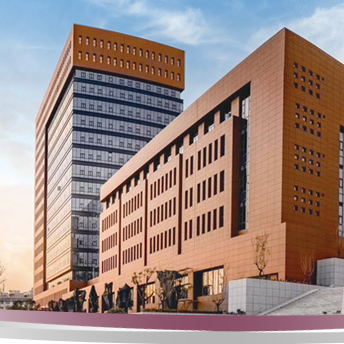
\includegraphics[width=1\linewidth]{hutb_building.png}
        \caption{bbb}
        \end{minipage}
    \end{subfigure}
    \caption{图片竖排多图横排布局}
    \label{f.csu_col_row}
\end{figure}

竖排多图横排布局如图\ref{f.csu_col_row}所示。注意看(a)、(b)编号与图关系


\section{横排多图竖排布局}

潮涌湘江阔,鹏翔天地宽。湖南工商大学正以习近平新时代中国特色社会主义思想为指引,秉持“新工科+新商科+新文科”与理科融合发展的思路,努力形成一流的理念、一流的目标、一流的标准、一流的质量、一流的机制,打造创新工商、人文工商、艺术工商、体育工商、数智工商、绿色工商、幸福工商,建设读书求知的好园地,乘高等教育改革奋进的东风,朝着创新型一流工商大学的愿景扬帆远航。

\begin{figure}[!htb]
    \centering
    \begin{subfigure}[t]{0.3\linewidth}
        \captionsetup{justification=centering} 
        \begin{minipage}[b]{1\linewidth}
        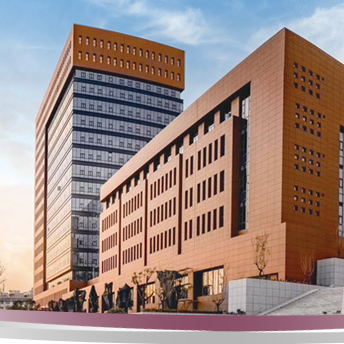
\includegraphics[width=0.45\linewidth]{hutb_building.png}
        \includegraphics[width=0.45\linewidth]{hutb_eim.png}
        \caption{}
        \end{minipage}
    \end{subfigure}\\
    \begin{subfigure}[t]{0.3\linewidth}
        \captionsetup{justification=centering} 
        \begin{minipage}[b]{1\linewidth}
        \includegraphics[width=0.45\linewidth]{hutb_eim.png}
        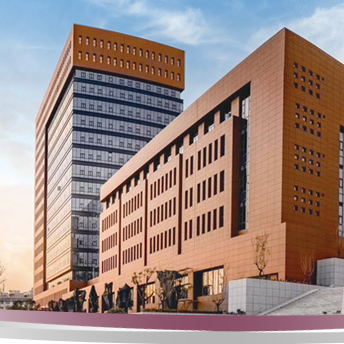
\includegraphics[width=0.45\linewidth]{hutb_building.png}
        \caption{}
        \end{minipage}
    \end{subfigure}
    \caption{图片横排多图竖排布局}
    \label{f.csu_row_col}
\end{figure}

横排多图竖排布局如图\ref{f.csu_row_col}所示。注意看(a)、(b)编号与图关系。

\newpage
%%%%%%%%%%%%%%%%%%%%%%%%%%%%%%%%图像插入示例%%%%%%%%%%%%%%%%


%%%%%%%%%%%%%%%%%%%%%%%%%%%%%%%%表格插入示例%%%%%%%%%%%%%%%%
%!TEX root = ../../csuthesis_main.tex
\chapter{表格插入示例}

\begin{table}[htb]
  \centering
  \caption{学校文件里对表格的要求不是很高,不过按照学术论文的一般规范,表格为三线表。}
  \label{T.example}
  \begin{tabular}{llllll}
  \hline
   & A  & B  & C  & D  & E \\
  \hline
1 	& 212 & 414 & 4 		& 23 & fgw	\\
2 	& 212 & 414 & v 		& 23 & fgw	\\
3 	& 212 & 414 & vfwe		& 23 & 嗯	\\
4 	& 212 & 414 & 4fwe		& 23 & 嗯	\\
5 	& af2 & 4vx & 4 		& 23 & fgw	\\
6 	& af2 & 4vx & 4 		& 23 & fgw	\\
7 	& 212 & 414 & 4 		& 23 & fgw	\\

\hline{}
\end{tabular}
\end{table}

\textbf{表格如表\ref{T.example}所示,latex表格技巧很多,这里不再详细介绍。}

潮涌湘江阔,鹏翔天地宽。湖南工商大学正以习近平新时代中国特色社会主义思想为指引,秉持“新工科+新商科+新文科”与理科融合发展的思路,努力形成一流的理念、一流的目标、一流的标准、一流的质量、一流的机制,打造创新工商、人文工商、艺术工商、体育工商、数智工商、绿色工商、幸福工商,建设读书求知的好园地,乘高等教育改革奋进的东风,朝着创新型一流工商大学的愿景扬帆远航。


\newpage

\chapter{公式插入示例}

潮涌湘江阔,鹏翔天地宽。湖南工商大学正以习近平新时代中国特色社会主义思想为指引,秉持“新工科+新商科+新文科”与理科融合发展的思路,努力形成一流的理念、一流的目标、一流的标准、一流的质量、一流的机制,打造创新工商、人文工商、艺术工商、体育工商、数智工商、绿色工商、幸福工商,建设读书求知的好园地,乘高等教育改革奋进的东风,朝着创新型一流工商大学的愿景扬帆远航。


\textbf{公式插入示例如公式(\ref{E.example})所示。}

\begin{equation}
\gamma_{x}=
\left\{
  \begin{array}{lr}
  0, & {\rm if}~~\;|x| \leq \delta \\
  x, & {\rm otherwise}
  \end{array}
\right.
\label{E.example}
\end{equation}


\newpage
%%%%%%%%%%%%%%%%%%%%%%%%%%%%%%%%表格插入示例%%%%%%%%%%%%%%%%


%%%%%%%%%%%%%%%%%%%%%%%%%%%%%%%%参考文献插入示例%%%%%%%%%%%%%%%%
%!TEX root = ../../csuthesis_main.tex
\chapter{引用文献标注}

文献标注和索引的处理一直是学术写作的一个麻烦事,特别是在word环境下。latex中我们只需要
编辑(或直接获取) BibTeX 格式索引文件然后在正文中使用\cs{cite} \cs{citet}等指令
进行引用标注就可以。下面介绍在文章中引用指令的具体使用方法。

\section{顺序编码}

根据学校要求,参考文献标注用中括号上标形式进行标注。使用方式与效果如下表所展示

\begin{tabular}{l@{\quad$\Rightarrow$\quad}l}
    \verb|\cite{knuth1984texbook}|               & \cite{knuth1984texbook}               \\
    \verb|\citet{knuth1984texbook}|              & \citet{knuth1984texbook}              \\
    \verb|\citep{knuth1984texbook}|              & \citep{knuth1984texbook}              \\
    % 暂不支持
    % \verb|\cite[42]{knuth1984texbook}|           & \cite[42]{knuth1984texbook}           \\
    \verb|\cite{knuth1984texbook,lamport1994latex}| & \cite{knuth1984texbook,lamport1994latex} \\
\end{tabular}

\section{获取BibTeX格式索引}

获取参考文献的 BibTeX 格式索引有两种方式

\begin{itemize}
    \item 通过Google Scholare或者百度学术等学术文献搜索引擎获取,自行编辑 .bib 文件
    \item 通过Zotero等学术文献整理软件,添加所有的引用文献至库中,导出对应的 .bib 文件
\end{itemize}

编译带参考文献的文章时,我们需要两次编译过程。我们提供了对应的自动化脚本,以及配合vscode latex插件的任务流程,
帮助模板使用者进行编译。

\section{参考文献插入示例}

LaTeX\cite{lamport1994latex}插入参考文献最方便的方式是使用bibliography\cite{pritchard1969statistical},大多数出版商的论文页面\cite{lamport1994latex,pritchard1969statistical}都会有导出bib格式参考文献的链接,把每个文献的bib放入``hutbthesis\_main.bib'',然后用bibkey即可插入参考文献。

潮涌湘江阔,鹏翔天地宽。湖南工商大学正以习近平新时代中国特色社会主义思想为指引,秉持“新工科+新商科+新文科”与理科融合发展的思路,努力形成一流的理念、一流的目标、一流的标准、一流的质量、一流的机制,打造创新工商、人文工商、艺术工商、体育工商、数智工商、绿色工商、幸福工商,建设读书求知的好园地,乘高等教育改革奋进的东风,朝着创新型一流工商大学的愿景扬帆远航。

\newpage




%%%%%%%%%%%%%%%%%%%%%%%%%%%%%%%%参考文献插入示例%%%%%%%%%%%%%%%%

%%%%%%%%%%%%%%%%%%%%%%%%%%%%%%%%总结插入示例%%%%%%%%%%%%%%%%
%!TEX root = ../../csuthesis_main.tex

%%%%%%%%%%%%%%%%%%%%%%%%%%%%%%%%总结插入示例%%%%%%%%%%%%%%%%



\chapter{选题背景与价值}

\section{选题价值}

智慧城市与智能交通发展背景下行人导航与控制系统在现代交通管理中作用重要。行人作为城市交通系统的重要组成部分其行为具有显著随机性和多样性给传统交通管理和路径规划方法带来诸多挑战,行人导航系统研究旨在通过实时路径优化与智能调控提升行人交通安全与出行效率。但传统导航方法多基于规则模型主要依赖静态预设参数,难以应对复杂动态环境中行人行为的快速变化,比如面对突发障碍物或密集交通流动时传统算法常无法快速调整路径规划或实时优化决策进而影响导航系统可靠性与安全性。

近年来人工智能技术快速发展,强化学习作为数据驱动的决策优化方法为行人导航领域提供全新思路,其通过智能体与环境交互学习最优策略能在动态环境中实现实时决策优化,特别适用于非线性非结构化的复杂场景。不过仅依靠强化学习技术难以全面解决行人导航问题,现实环境中数据采集的高成本高风险特性在实际应用中极大限制了强化学习的训练与推广。

本研究基于 Carla 利用虚幻引擎这一高仿真度虚拟场景构建平台提供了解决实际环境数据采集困难的理想工具,该引擎既能生成复杂多样的动态环境也能模拟真实场景中行人行为的随机性和多样性,为强化学习智能体的训练与测试提供安全低成本的实验平台。如通过虚幻引擎模拟十字路口复杂交通场景可逼真再现行人与车辆的动态交互,为强化学习算法的优化与验证创造实验条件,且其支持生成视觉、惯性、语义信息等多种传感器数据进一步丰富了强化学习的训练数据来源。

本研究结合虚拟仿真技术和强化学习算法解决行人导航核心问题,包括精准建模动态环境下行人行为,行人行为受交通信号、周围车辆动态变化及其他行人行为等多种因素影响,建立能真实反映不同环境中行人决策逻辑的高精度行人行为模型是首要难题;高效结合虚拟仿真与强化学习,强化学习有效性依赖训练环境质量,虚幻引擎仿真能力为训练高效智能体提供可能,但设计能充分利用虚幻引擎生成的多样化数据的高效强化学习算法亟待解决;平衡路径规划效率与行人安全性,行人导航系统要提高路径规划效率并优先考虑行人安全,如在交通高峰期复杂场景中找到安全高效路径是研究重点。

智慧交通系统发展对行人导航系统提出更高要求,既需与车辆、交通信号灯等其他交通参与者无缝协作以优化交通系统运行效率,随着多智能体技术发展,行人导航系统研究也从单一智能体优化转向多智能体协作,通过多智能体协同作用提升导航效率与安全性是未来重要研究方向。

本研究引入虚幻引擎仿真能力与强化学习自适应策略优化能力试图突破上述问题,虚幻引擎的逼真场景和多样化数据为复杂行为建模和智能体训练提供支持,强化学习算法自适应优化能力使智能体可快速适应复杂动态环境变化,两者结合能为行人导航系统提供新理论和技术支撑,在智能交通、自动驾驶和城市规划等领域有广泛应用潜力。

\section{文献综述}

近年来强化学习与虚拟仿真技术在智能交通和行人导航领域研究取得显著进展,从强化学习在行人导航中的应用、虚幻引擎在智能体训练中的作用以及行人导航的挑战与发展趋势三方面进行综述。

\subsection{强化学习在行人导航中的应用}

强化学习(Reinforcement Learning, RL)是一种通过智能体与环境交互学习最优策略的方法,近年来在交通系统优化和行人导航中得到了广泛应用。与传统路径规划方法相比,强化学习不仅可以应对动态环境,还能通过不断训练提高系统性能,展现了较高的自适应性和优化能力。强化学习技术在交通信号控制取得重要成果,钱立军等\cite{qian2024sac}基于 SAC 算法优化多交叉口交通信号控制提升交通通行效率,为动态环境复杂信号调度提供新思路,Wei 等\cite{wei2021survey}综述强化学习在交通信号控制研究进展指出深度强化学习(Deep Reinforcement Learning, DRL)解决非线性优化问题优势适用于实时动态交通场景;在路径规划领域应用广泛,陶幸等\cite{tao2024motion}提出基于惯性传感器免对准动作捕捉方法为动态场景行人行为建模提供技术支持,Chen 等\cite{chen2018ionet}结合深度学习与强化学习技术设计基于因果推理路径优化方法引入因果关系提升智能体在动态环境适应能力;深度强化学习为路径规划研究注入新动力,Mnih 等\cite{mnih2013dqn}首次提出深度 Q 学习(Deep Q - Learning, DQN)算法将深度神经网络引入强化学习框架提升其在高维状态空间表现能力;在多智能体协作问题广泛研究,Lian 等\cite{lian2023inverseql}设计基于离线 Q 学习多智能体协作算法解决复杂动态场景全局优化问题。

\subsection{虚幻引擎在智能体训练中的作用}

虚幻引擎(Unreal Engine)作为高仿真虚拟场景构建工具为复杂动态环境下强化学习算法训练和验证提供高效实验平台,借由强大虚拟仿真能力和多样化场景支持成为智能体训练测试重要工具。

1. \textbf{虚幻引擎在视觉导航研究中的应用:} 虚幻引擎在视觉导航研究应用广泛,Mourikis 等\cite{mourikis2007msckf}结合虚幻引擎构建视觉惯性导航系统并通过多状态约束卡尔曼滤波(MSCKF)算法优化路径规划,Campos 等\cite{campos2021orbslam3}提出的 ORB-SLAM3 算法利用虚拟场景数据显著提升视觉建图与定位的鲁棒性和精度为复杂动态环境中的导航提供有力支持。

2. \textbf{虚幻引擎在路径规划中的贡献:} 虚幻引擎于路径规划研究表现重要作用,Guo 等\cite{guo2020pdr}结合虚幻引擎动态仿真能力提出基于 PDR/UWB 融合的导航系统用于复杂环境行人路径优化,Wang 等\cite{wang2023llio}通过虚幻引擎构建高仿真交通场景训练强化学习智能体路径规划策略验证其在强化学习训练中的高效性和低成本特性。

3. \textbf{虚幻引擎与目标检测的结合:} 虚幻引擎还被用于目标检测与路径规划结合研究,Redmon 等\cite{redmon2017yolo9000}通过虚幻引擎生成增强数据训练 YOLO 目标检测模型提高目标检测在复杂场景中的表现能力,Simonyan 和 Zisserman 等\cite{simonyan2014action}进一步研究虚幻引擎对深度学习模型的优化作用为复杂交通场景下的行为预测提供理论支持。 

4. \textbf{虚幻引擎在多智能体协作中的应用:} 虚幻引擎的仿真能力在多智能体协作研究中广泛应用,Bochkovskiy 等\cite{bochkovskiy2020yolov4}开发基于虚幻引擎的交通流量仿真工具验证多智能体协作算法有效性,Campos 等\cite{campos2021orbslam3}通过虚拟场景数据验证智能体在多智能体协作场景中的优化表现为行人导航系统的多智能体研究提供重要支持。

虚幻引擎为强化学习算法设计训练与验证提供有力支持,在视觉导航路径规划与多智能体协作中的应用展现巨大潜力。

\subsection{行人导航的挑战与发展趋势}

行人导航技术虽取得显著进展但在复杂动态环境中仍存复杂行为建模、动态环境适应性及多智能体协作优化等诸多挑战。

1. \textbf{行人行为的复杂建模:} 行人行为具显著多样性与随机性,赵靖等\cite{zhao2014crossing}提出基于动态信号优化的行人过街模型通过行为建模提升信号控制效率与安全性,Foxlin 等\cite{foxlin2005tracking}设计基于惯性传感器的行人轨迹跟踪方法为复杂行为建模提供技术支持。

2. \textbf{动态环境的实时适应:} 动态环境不确定性对导航系统提出更高要求,Herath 等\cite{herath2020ronin}通过视觉信号优化路径规划使智能体实时适应动态障碍物变化,Wang 等\cite{wang2013densetrajectory}提出基于强化学习的信号优化方法在动态环境中提升系统鲁棒性。

3. \textbf{多智能体协作的优化:} 复杂交通场景中多智能体协作优化问题尤为重要,Lian 等\cite{lian2023inverseql}通过强化学习实现多智能体高效协作提高全局路径规划效率,Campos 等\cite{campos2021orbslam3}利用虚幻引擎验证多智能体协作优化算法在复杂场景中的应用价值。

4. \textbf{未来研究趋势:} 未来行人导航研究将朝以下方向发展:基于多源数据的复杂行为建模与优化;提升强化学习智能体在动态环境中的泛化能力;多智能体协作优化在虚拟仿真环境中的深度应用。

%!TEX root = ../../csuthesis_main.tex
\chapter{图表示例}

\section{图片与布局}

\subsection{插图}

图片可以通过\cs{includegraphics}指令插入,我们建议模板使用者将文章所需插入的图片源问卷放置在 images 目录中,
另外,矢量图片应使用PDF格式,位图照片则应使用JPG格式(LaTeX不支持TIFF格式)。具有透明背景的栅格图可以使用PNG格式。

下面是一个简单的插图示例。

\begin{figure}[hbt]
    \centering
    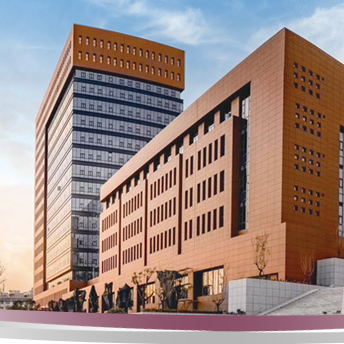
\includegraphics[width=0.3\linewidth]{hutb_building.png}
    \caption{插图示例}
    \label{f.example}
\end{figure}


如果一个图由多个分图(子图)组成,应通过(a),(b),(c)进行标识并附注在分图(子图下方)。
目前子图标识不居中问题没有解决,预计下个版本修复。

\subsection{横向布局}

模板提供常见的图片布局,比如单图布局\ref{f.example},另外还有横排布局如下:

\begin{figure}[!htb]
    \centering
    \begin{subfigure}[t]{0.24\linewidth}
        \begin{minipage}[b]{1\linewidth}
        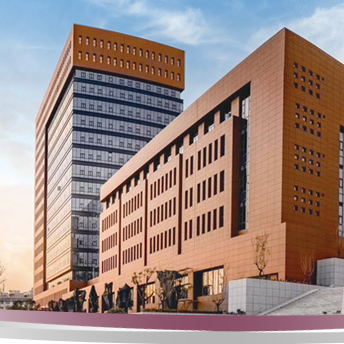
\includegraphics[width=1\linewidth]{hutb_building.png}
        \caption{test}
        \end{minipage}
    \end{subfigure}
    \begin{subfigure}[t]{0.24\linewidth}
        \begin{minipage}[b]{1\linewidth}
        \includegraphics[width=1\linewidth]{hutb_eim.png}
        \caption{test}
        \end{minipage}
    \end{subfigure}
    \begin{subfigure}[t]{0.24\linewidth}
        \begin{minipage}[b]{1\linewidth}
        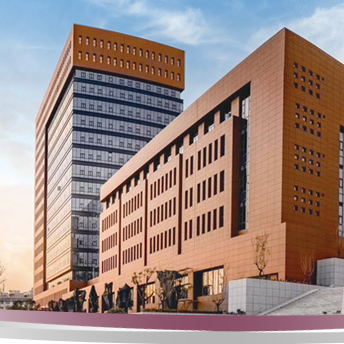
\includegraphics[width=1\linewidth]{hutb_building.png}
        \caption{test}
        \end{minipage}
    \end{subfigure}
    \begin{subfigure}[t]{0.24\linewidth}
        \begin{minipage}[b]{1\linewidth}
        \includegraphics[width=1\linewidth]{hutb_eim.png}
        \caption{test}
        \end{minipage}
    \end{subfigure}
    \caption{图片横排布局示例}
    \label{f.row}
\end{figure}

\section{纵向布局}

纵向布局如图\ref{f.col}

\begin{figure}[!htb]
    \centering
    \begin{subfigure}[t]{0.15\linewidth}
        \captionsetup{justification=centering} %ugly hacks
        \begin{minipage}[b]{1\linewidth}
        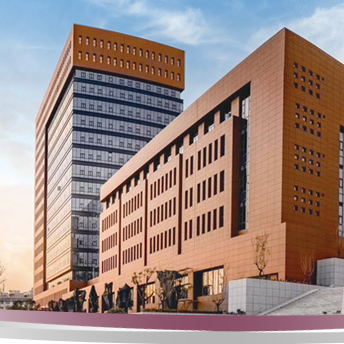
\includegraphics[width=1\linewidth]{hutb_building.png}
        \caption{test}
        \end{minipage}
    \end{subfigure}\\
    \begin{subfigure}[t]{0.15\linewidth}
        \captionsetup{justification=centering} %ugly hacks
        \begin{minipage}[b]{1\linewidth}
        \includegraphics[width=1\linewidth]{hutb_eim.png}
        \caption{test}
        \end{minipage}
    \end{subfigure}
    \caption{图片纵向布局示例}
    \label{f.col}
\end{figure}

\section{竖排多图横排布局}

\begin{figure}[!htb]
    \centering
    \begin{subfigure}[t]{0.13\linewidth}
        \captionsetup{justification=centering} 
        \begin{minipage}[b]{1\linewidth}
        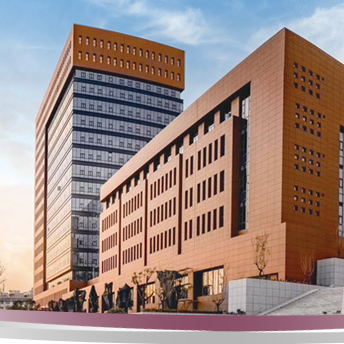
\includegraphics[width=1\linewidth]{hutb_building.png} 
        \vspace{-1ex} \vfill
        \includegraphics[width=1\linewidth]{hutb_eim.png}
        \caption{aaa}
        \end{minipage}
    \end{subfigure}
    \begin{subfigure}[t]{0.13\linewidth}
        \captionsetup{justification=centering} 
        \begin{minipage}[b]{1\linewidth}
        \includegraphics[width=1\linewidth]{hutb_eim.png} 
        \vspace{-1ex} \vfill
        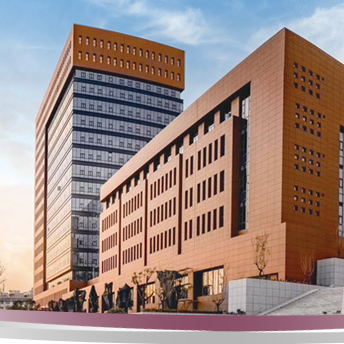
\includegraphics[width=1\linewidth]{hutb_building.png}
        \caption{bbb}
        \end{minipage}
    \end{subfigure}
    \caption{图片竖排多图横排布局}
    \label{f.csu_col_row}
\end{figure}

竖排多图横排布局如图\ref{f.csu_col_row}所示。注意看(a)、(b)编号与图关系


\section{横排多图竖排布局}

潮涌湘江阔,鹏翔天地宽。湖南工商大学正以习近平新时代中国特色社会主义思想为指引,秉持“新工科+新商科+新文科”与理科融合发展的思路,努力形成一流的理念、一流的目标、一流的标准、一流的质量、一流的机制,打造创新工商、人文工商、艺术工商、体育工商、数智工商、绿色工商、幸福工商,建设读书求知的好园地,乘高等教育改革奋进的东风,朝着创新型一流工商大学的愿景扬帆远航。

\begin{figure}[!htb]
    \centering
    \begin{subfigure}[t]{0.3\linewidth}
        \captionsetup{justification=centering} 
        \begin{minipage}[b]{1\linewidth}
        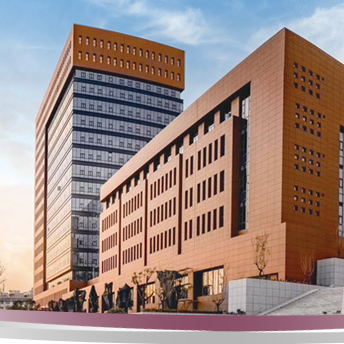
\includegraphics[width=0.45\linewidth]{hutb_building.png}
        \includegraphics[width=0.45\linewidth]{hutb_eim.png}
        \caption{}
        \end{minipage}
    \end{subfigure}\\
    \begin{subfigure}[t]{0.3\linewidth}
        \captionsetup{justification=centering} 
        \begin{minipage}[b]{1\linewidth}
        \includegraphics[width=0.45\linewidth]{hutb_eim.png}
        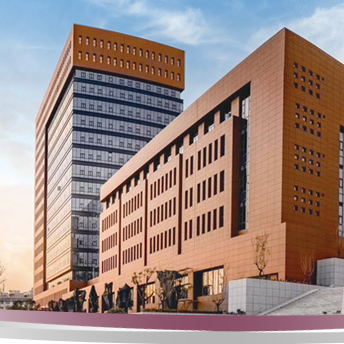
\includegraphics[width=0.45\linewidth]{hutb_building.png}
        \caption{}
        \end{minipage}
    \end{subfigure}
    \caption{图片横排多图竖排布局}
    \label{f.csu_row_col}
\end{figure}

横排多图竖排布局如图\ref{f.csu_row_col}所示。注意看(a)、(b)编号与图关系。

\newpage
%!TEX root = ../../csuthesis_main.tex
\chapter{表格插入示例}

\begin{table}[htb]
  \centering
  \caption{学校文件里对表格的要求不是很高,不过按照学术论文的一般规范,表格为三线表。}
  \label{T.example}
  \begin{tabular}{llllll}
  \hline
   & A  & B  & C  & D  & E \\
  \hline
1 	& 212 & 414 & 4 		& 23 & fgw	\\
2 	& 212 & 414 & v 		& 23 & fgw	\\
3 	& 212 & 414 & vfwe		& 23 & 嗯	\\
4 	& 212 & 414 & 4fwe		& 23 & 嗯	\\
5 	& af2 & 4vx & 4 		& 23 & fgw	\\
6 	& af2 & 4vx & 4 		& 23 & fgw	\\
7 	& 212 & 414 & 4 		& 23 & fgw	\\

\hline{}
\end{tabular}
\end{table}

\textbf{表格如表\ref{T.example}所示,latex表格技巧很多,这里不再详细介绍。}

潮涌湘江阔,鹏翔天地宽。湖南工商大学正以习近平新时代中国特色社会主义思想为指引,秉持“新工科+新商科+新文科”与理科融合发展的思路,努力形成一流的理念、一流的目标、一流的标准、一流的质量、一流的机制,打造创新工商、人文工商、艺术工商、体育工商、数智工商、绿色工商、幸福工商,建设读书求知的好园地,乘高等教育改革奋进的东风,朝着创新型一流工商大学的愿景扬帆远航。


\newpage

\chapter{公式插入示例}

潮涌湘江阔,鹏翔天地宽。湖南工商大学正以习近平新时代中国特色社会主义思想为指引,秉持“新工科+新商科+新文科”与理科融合发展的思路,努力形成一流的理念、一流的目标、一流的标准、一流的质量、一流的机制,打造创新工商、人文工商、艺术工商、体育工商、数智工商、绿色工商、幸福工商,建设读书求知的好园地,乘高等教育改革奋进的东风,朝着创新型一流工商大学的愿景扬帆远航。


\textbf{公式插入示例如公式(\ref{E.example})所示。}

\begin{equation}
\gamma_{x}=
\left\{
  \begin{array}{lr}
  0, & {\rm if}~~\;|x| \leq \delta \\
  x, & {\rm otherwise}
  \end{array}
\right.
\label{E.example}
\end{equation}


\newpage
%!TEX root = ../../csuthesis_main.tex
\chapter{引用文献标注}

文献标注和索引的处理一直是学术写作的一个麻烦事,特别是在word环境下。latex中我们只需要
编辑(或直接获取) BibTeX 格式索引文件然后在正文中使用\cs{cite} \cs{citet}等指令
进行引用标注就可以。下面介绍在文章中引用指令的具体使用方法。

\section{顺序编码}

根据学校要求,参考文献标注用中括号上标形式进行标注。使用方式与效果如下表所展示

\begin{tabular}{l@{\quad$\Rightarrow$\quad}l}
    \verb|\cite{knuth1984texbook}|               & \cite{knuth1984texbook}               \\
    \verb|\citet{knuth1984texbook}|              & \citet{knuth1984texbook}              \\
    \verb|\citep{knuth1984texbook}|              & \citep{knuth1984texbook}              \\
    % 暂不支持
    % \verb|\cite[42]{knuth1984texbook}|           & \cite[42]{knuth1984texbook}           \\
    \verb|\cite{knuth1984texbook,lamport1994latex}| & \cite{knuth1984texbook,lamport1994latex} \\
\end{tabular}

\section{获取BibTeX格式索引}

获取参考文献的 BibTeX 格式索引有两种方式

\begin{itemize}
    \item 通过Google Scholare或者百度学术等学术文献搜索引擎获取,自行编辑 .bib 文件
    \item 通过Zotero等学术文献整理软件,添加所有的引用文献至库中,导出对应的 .bib 文件
\end{itemize}

编译带参考文献的文章时,我们需要两次编译过程。我们提供了对应的自动化脚本,以及配合vscode latex插件的任务流程,
帮助模板使用者进行编译。

\section{参考文献插入示例}

LaTeX\cite{lamport1994latex}插入参考文献最方便的方式是使用bibliography\cite{pritchard1969statistical},大多数出版商的论文页面\cite{lamport1994latex,pritchard1969statistical}都会有导出bib格式参考文献的链接,把每个文献的bib放入``hutbthesis\_main.bib'',然后用bibkey即可插入参考文献。

潮涌湘江阔,鹏翔天地宽。湖南工商大学正以习近平新时代中国特色社会主义思想为指引,秉持“新工科+新商科+新文科”与理科融合发展的思路,努力形成一流的理念、一流的目标、一流的标准、一流的质量、一流的机制,打造创新工商、人文工商、艺术工商、体育工商、数智工商、绿色工商、幸福工商,建设读书求知的好园地,乘高等教育改革奋进的东风,朝着创新型一流工商大学的愿景扬帆远航。

\newpage




%!TEX root = ../../csuthesis_main.tex


% % 主文件有代码去掉页眉章节编号的“.”,但这会因为bug导致无编号章节显示一个错误编号,所以这里在无编号章节之前再次重定义sectionmark。
% \renewcommand{\sectionmark}[1]{\markright{#1}}


%%%%%%%%%%%%%%%%%%%%%%%%%%%%%%%%%%%%%%%%%%%%%%%%%%
% 致谢
%
% 存储在\content\acknowledgements.tex文件中
% 根据本科生院的要求,致谢应该在参考文献的前面,不编章号,而附录应该位于参考文献后。
%%%%%%%%%%%%%%%%%%%%%%%%%%%%%%%%%%%%%%%%%%%%%%%%%%
%!TEX root = ../csuthesis_main.tex
\begin{acknowledgements} 

感谢制作出中南大学本科学位论文 LaTeX 模板的edwardzcn。

感谢制作出中南大学博士学位论文 LaTeX 模板的郭大侠@CSGrandeur。

感谢添加本科学位论文样式支持的@BlurryLight。

感谢帮助重构项目并进行测试的@burst-bao以及为独立使用LaTeX进行毕业论文写作提供宝贵经验的16级的姜析阅学长。

感谢 CTeX-kit 提供了 LaTeX 的中文支持。

感谢上海交通大学学位论文 LaTeX 模板的维护者们 @sjtug 和清华大学学位论文 LaTeX 模板的维护者们 @tuna 给予的宝贵设计经验。

感谢所有为模板贡献过代码的同学们!

\end{acknowledgements}


%%%%%%%%%%%%%%%%%%%%%%%%%%%%%%%%%%%%%%%%%%%%%%%%%%
% 参考文献
%
% 存储在\content\acknowledgements.tex文件中
% 根据本科生院的要求,致谢应该在参考文献的前面,不编章号,而附录应该位于参考文献后。
% 有待修复
%%%%%%%%%%%%%%%%%%%%%%%%%%%%%%%%%%%%%%%%%%%%%%%%%%
% \section{参考文献} % bibliography会自动显示参考文献四个字
\addcontentsline{toc}{chapter}{参考文献} % 由于参考文献不是chapter,这句把参考文献加入目录
% \nocite{*} % 该命令用于显示全部参考文献,即使文中没引用
% cls文件中已经引入package,这里不需要调用 \bibliographystyle 了。
%\bibliographystyle{gbt7714-2005}
%\bibliography{reference}

\printbibliography

%\bibliography{hutbtheisi_main}
\newpage


%%%%%%%%%%%%%%%%%%%%%%%%%%%%%%%%%%%%%%%%%%%%%%%%%%
% 附录部分
%
% 根据学校要求,正文中不应出现长篇幅的代码段或公式推证
% 应单独放置在正文后的附录部分
%%%%%%%%%%%%%%%%%%%%%%%%%%%%%%%%%%%%%%%%%%%%%%%%%%

% https://www.zhihu.com/question/29413517/answer/44358389 %
% 说明如下:
% secnumdepth 这个计数器是 LaTeX 标准文档类用来控制章节编号深度的。
% 在 article 中,这个计数器的值默认是 3,对应的章节命令是 \subsubsection。
% 也就是说,默认情况下,article 将会对 \subsubsection 及其之上的所有章节标题进行编号,也就是 \part, \section, \subsection, \subsubsection。LaTeX 标准文档类中,最大的标题是 \part。它在 book 和 report 类中的层级是「-1」,在 article 类中的层级是「0」。这里,我们在调用 \appendix 的时候将计数器设置为 -2,因此所有的章节命令都不会编号了。不过,一般还是会保留 \part 的编号的。所以在实际使用中,将它设置为 0 就可以了。

% 在修改过程中请注意不要破环命令的完整性

% \renewcommand\appendix{\setcounter{secnumdepth}{-2}}
\appendix
%!TEX root = ../csuthesis_main.tex
% \begin{appendixs} % 无章节编号
\chapter{附录代码}

附录部分用于存放这里用来存放不适合放置在正文的大篇幅内容、典型如代码、图纸、完整数学证明过程等内容。

\section{堆溢出检测算法}

\begin{algorithm}[h]
    \caption{堆溢出检测算法}\label{alg:ovf}
    \begin{algorithmic}[1]
        \IF {$\beta \in \mathbb{N^{*}} \land \Delta_\beta = \Delta_{\beta - 1} \land \beta < S$}
            \STATE 正常写入
        \ELSIF {$\beta \in \mathbb{N^{*}} \land \Delta_\beta \neq \Delta_{\beta - 1} \land \beta \geq S$}
            \STATE 发生堆溢出
        \ENDIF
    \end{algorithmic}
\end{algorithm}

\section{KMP算法C++描述}

% \begin{minted}[linenos]{c}
\begin{lstlisting}
    const int maxn=2e5+5; 
    int nt[maxn];
    int aa[maxn],bb[maxn];
    int a[maxn],b[maxn];
    int n;
    //参数为模板串和next数组
    //字符串均从下标0开始
    void kmpGetNext(int *s,int *Next)
    {
        Next[0]=0;
    //    int len=strlen(s);
        for(int i=1,j=0;i<n;i++)
        {
            while(j&&s[i]!=s[j]) j=Next[j];
            if(s[i]==s[j]) j++;
            Next[i+1]=j;
        }
    //    Next[len]=0;
    }
    int kmp(int *ss,int *s,int *Next)
    {
        kmpGetNext(s,Next);
    //  调试输出Next数组
    //	int len=strlen(s);
    //	for(int i=0;i<=n;i++)
    //		cout<<Next[i]<<" ";
    //	cout<<endl; 
    
    //    int ans=0;
    //    int len1=strlen(ss);
    //    int len2=strlen(s);
        for(int i=0,j=0;i<2*n;i++)  //倍长 
        {
            while(j&&ss[i%n]!=s[j])j=Next[j];
            if(ss[i%n]==s[j]) j++;
            if(j==n){
                return 1;
            }
               
        }
        return 0;
    }
    int main(void)
    {
        while(cin>>n)
        {
            memset(a,0,sizeof(a));
            memset(b,0,sizeof(b));
            rep(i,0,n) cin>>aa[i];
            rep(i,0,n) cin>>bb[i];
            sort(aa,aa+n);
            sort(bb,bb+n);
            rep(i,0,n-1){
                a[i]=aa[i+1]-aa[i];
                b[i]=bb[i+1]-bb[i];
            }
            a[n-1]=360000+aa[0]-aa[n-1];
    //		rep(i,0,n) cout<<a[i]<<" ";
    //		cout<<endl;
            b[n-1]=360000+bb[0]-bb[n-1];
    //		rep(i,0,n) cout<<b[i]<<" ";
    //		cout<<endl;
            if(kmp(a,b,nt))
                cout<<"possible"<<endl;
            else cout<<"impossible"<<endl;
        }
        return 0;
    }
\end{lstlisting}
% \end{minted}

\chapter{康托尔辩辞录:数学的自由与制约}

(录自康托尔:《一般集合论基础》,1883)

数学在其发展中是完全自由的,它只受下述自明的关注所制约,即它的概念既要内在地不存在矛盾,还要参与确定与此前形成的,已经存在着地和已被证明地概念之关系(借助定义贯串起来)。特别地,在引入新数时,数学只遵循:在给出它们地定义时使之具有某种确定性,并且在某些情况下,使之与老数有某种关系,在特定地场合中这种关系一定会使它们(新数和老数)互相区别开来,只要一个数满足这些条件,数学只能而且必须把它看作是存在的和实在的东西,这正是我……关于为什么必须把有理数、无理数和复数看作与有限正整数一样是实在的所建议的理由。

我相信,没有必要害怕,许多人是害怕,这些原则含有对于科学的危险,一方面,实行造出新数的自由必须服从所设计的条件,但这些条件给任意性留下的活动空间是非常小的。而且,每一数学概念在其自身之中也带有必要的矫正物;如果它没有收获也不合适(它的无用很快就会表明这一点),那么它将由于没有成功而被丢弃。另一方面,在我看来,对于数学研究工作的任何多余的限制只会随之而带来更大的危险,由于实际上并没有任何理由可说明它是由科学的本质推断出来的,它的危险就更大了,而数学的本质恰恰在于它的自由。

如果高斯、柯西、阿贝尔、雅可比、狄利克雷、魏尔斯特拉斯、埃尔米特和黎曼总是被束缚而拿他们的新想法去臣服于形而上学的控制,那么,我们今日就不可能为现代函数论的雄伟建筑而高兴,现代函数论的设计和矗立是完全自由的,毫无短视的瞬间目的……。如果福克斯、庞加莱和其他许多杰出的智者受外来影响所包围和限制,我们就会见不到他们带给微分方程论的巨大的推动,还有,如果枯莫尔不是斗胆地(大有仿效者)把所谓的“理想”数引入数论,我们今天也无从去羡慕钦佩克罗内克和戴德金在代数和算术上十分重要和杰出的工作。

因此,如已说明的,数学是要脱离形而上学的桎梏而完全自由地发展 \dots



% \end{appendixs}



\end{document}
